%TODO Name Header passen nicht

\renewcommand{\theauthor}{Matthias Franz}
\chapter{iCal}
\label{sec:iCal}
Dieses Kapitel befasst sich mit dem iCal-Dateiformat welches einen großen Teil in dieser Diplomarbeit einnimmt. Es wird behandelt wie eine iCal-Datei aufgebaut ist und weshalb iCal in diesem Projekt verwendet wurde.

\section{Was ist iCal?}
\label{sec:wasIstiCal?}
iCal ist ein Dateiformat, welches dazu verwendet wird um Kalender zu speichern. Fast jede Kalenderanwendung verwendet zur Speicherung und Manipulation ihrer Kalender iCal. Als Datei hat eine iCal-Datei die Endung .ics. Eine .ics Datei ist von Menschen lesbar und leicht veränderbar, was die Arbeit mit iCal-Dateien um einiges vereinfacht. \\
iCal ist ein MIME-Typ, dies ermöglicht es iCal-Dateien über jegliche Methoden zu versenden.\\vgl. \textcite{iCalDocumentation} 

\section{Warum wurde iCal verwendet?}
\label{sec:warumWurdeiCalVerwendet?}
iCal wurde verwendet, da der Großteil der Kalenderprogramme dieses Format verwenden und es viele Ressourcen rund um iCal gibt, was den Umgang damit deutlich vereinfacht. Weiters sind die Grundlagen einer iCal-Datei wegen des einfachen Aufbaues schnell verstanden.\\
iCal hat ein ATTACH Attribut welches einem erlaubt Dateien an einen Termin anzuhängen. Es gibt die Möglichkeit Dateien als Binär-Dateien oder als URLs zu FTP-Servern in das Attribut zu speichern. Da Binär-Dateien große Speichermengen verursachen wurde in diesem Projekt, um Speicher zu sparen, die Variante mit den URLs zu FTP-Servern verwendet. Weiters werden die URLs zu den FTP-Servern nicht in das ATTACH-Attribut geschrieben, sondern in die Beschreibung des Artikels, da oft externe Unternehmen auf Kalender zugreift und somit eine Kurzbeschreibung über die angegebene Datei angeben werden kann. Wenn auf die Dateien über einen FTP-Server zugegriffen wird, benötigen Benutzer Zugriff auf den FTP-Server. Dies ist eine weitere Sicherheitsmaßnahme, denn so werden auch wenn jemand Zugriff auf einen Kalender bekommt nur die Termine angezeigt. Auf die Dateien welche am FTP-Server liegen kann nur mit den richtigen Zugriffsdaten zugegriffen werden.\\
Die meisten Kalenderanwendungen haben von Haus aus eine Funktion um Kalender im iCal-Format zu exportieren oder um Kalender im iCal-Format zu importieren. Weiters haben die meisten Kalenderapplikationen die Funktion, dass Kalender als URL einbinden kann. Durch diese Funktion kann der URL welcher vom Webservice generiert wird, in ein Kalenderprogramm einbinden.
\\
Wenn allerdings versucht wird, ein iCal-Format per URL einzubinden und dieser URL ein localhost ist, erlauben Kalenderprogramme die Integration der iCal-Datei nicht.

\section{Aufbau einer iCal-Datei}
\label{sec:aufbauEineriCalDatei}
iCal-Dateien sind in einer Key-Value-Struktur aufgebaut, wobei sich jedes Key-Value-Paar in einer eigenen Zeile befindet. Eine iCal-Datei kann aus mehreren Kalendern bestehen und ein Kalender kann wiederum aus mehreren Objekten bestehen. Die Wichtigsten sind: Event-, To-Do- und Journal-Elemente, welche genauer im Kapitel \ref{sec:keywords}.\\\\
\texttt{BEGIN:VCALENDAR\\
 VERSION:2.0\\
 PRODID:-//hacksw/handcal//NONSGML v1.0//EN\\
 BEGIN:VEVENT\\
 UID:19970610T172345Z-AF23B2@example.com\\
 DTSTAMP:19970610T172345Z\\
 DTSTART:19970714T170000Z\\
 DTEND:19970715T040000Z\\
 SUMMARY:Bastille Day Party\\
 END:VEVENT\\
 END:VCALENDAR}\\\\
Eine .ics Datei ist hierarchisch aufgebaut. Eine Datei muss mit BEGIN:VCALENDAR beginnen. Wenn ein Kalender mit BEGIN:VCALENDAR begonnen wird, muss er wie jedes andere Element einer iCal-Datei auch wieder geschlossen werden um die beinhalteten Elemente einordnen zu können. Die VCALENDAR Eigenschaft kann viele Attribute haben welche das Verhalten des Kalenders verändern. Die meisten dieser Attribute sind allerdings nicht für diese Diplomarbeit relevant und wurden deshalb weggelassen. In einem VCALENDAR Element kann dann entweder ein Event-, To-Do oder Journal-Element erstellen. Es gibt noch weiter erstellbare Elemente, diese sind aber für diese Diplomarbeit nicht von Relevanz. Wie im Beispiel angeführt wird im VCALENDAR ein VEVENT erstellt. Dieses VEVENT muss dann wie der VCALENDAR und alle anderen Attribute wieder geschlossen werden. Im Beispiel ist erkenntlich, dass Events auch mehrere Attribute haben welches das Verhalten des Events ändern. Zum Beispiel SUMMARY, beschreibt was in der Kalenderapplikation in diesem Termin stehen würde.\\
Eine iCal-Datei besteht aus einem Key-Value Paar pro Zeile, im iCal-Jargon nennt man eine Zeile Content-Line. Eine Content-Line sollte nicht länger als 75 octets sein. Eine Content-Line kann an jeder beliebigen Stelle mit einem CLRF in zwei oder mehrere Zeilen geteilt werden, indem in der folgenden Zeile am Beginn eine Leerzeile einfügt. Für jede weitere Teilung wird ein weiteres Leerzeichen am Beginn der Zeile benötigt. \\\\
Zum Beispiel kann\vspace*{2mm}\\
\texttt{DESCRIPTION:This is a long description that exists on a long line.}\vspace*{2mm}\\als\vspace*{2mm}\\
\texttt{DESCRIPTION:This is a lo\\ 
\phantom{x}\hspace{1ex}ng description\\  
\phantom{x}\hspace{2ex}that exists on a long line.}\\\\
dargestellt werden.\vspace*{2mm}\\
Manche iCal-Attribute können mehr als nur einen Wert für den dementsprechenden Schlüssel haben. Diese einzelnen Elemente sind dann mit einen Komma getrennt. Wenn ein Schlüssel mehrere verschiedene Attribute enthält, werden diese mit einem Strichpunkt getrennt. Wenn ein Wert eines Attributes ein Komma oder einen Strichpunkt enthält, dann muss dass Komma oder der Strichpunkt unter Anführungszeichen gesetzt werden.\\\\
Ein Beispiel für die Trennung von Daten einer Liste in einem Schlüssel:\vspace*{2mm}\\
\texttt{RDATE;VALUE=DATE:19970304,19970504,19970704,19970904}\vspace*{2mm}\\
Wie in diesem Beispiel erkenntlich ist, wurden die Werte für das Datum mit Kommas getrennt.\\\\
Ein Beispiel für die Trennung von mehreren Attributen innerhalb eines Schlüssels:\vspace*{2mm}\\
\texttt{ATTENDEE;RSVP=TRUE;ROLE=REQ-PARTICIPANT:mailto:
jsmith@example.com}\vspace*{2mm}\\Es ist erkenntlich, dass die verschiedenen Attribute wie RSVP und ROLE mit einem Strichpunkt getrennt worden sind. Genaueres zum ATTENDEE-Attribut im Kapitel \ref{sec:attendee}. 
\\vgl. \textcite{iCalDocumentation} 

\pagebreak
\renewcommand{\theauthor}{Dario Wagner}
% TODO: Erklärung der verwendeten Keywords
% TODO: Zitate auf die Seite machen: https://www.kanzaki.com/docs/ical/
\section{Keywords}
\label{sec:keywords}
Unter dieser Überschrift werden die in der Diplomarbeit verwendeten iCal-Keywords aufgelistet und erklärt. Am Ende der Auflistung folgt ein Beispiel welches alle genannten Keywords enthält. 
\subsection{VCALENDAR}
\label{sec:vCalendar} 
Die Komponente ''VCALENDAR'' tritt nur im Zusammenhang mit ''BEGIN:'' oder ''END:'' auf. Sie gibt an wann ein Kalender beginnt und wann er aufhört. Jede weiter Komponente zwischen einem ''BEGIN:VCALENDAR'' und ''END:VCALENDAR'' gehört also zu einem Kalender. Ein Kalender kann Events, Termine, und ''ToDo's'', noch zu erldigende Aufgaben, enthalten. Ein Kalender ist also eine Gruppe von Terminen oder anderen Einträgen. 
\subsection{VEVENT}
\label{sec:vEvent} 
Ein Event ist wie in \ref{sec:vCalendar} erwähnt ein Termin. Jeder Termin kann einen Alarm \ref{sec:vAlarm} enthalten. Das Event im Kalender kann auch unter anderem als eine regelmäßige Erinnerung im Kalender spezifiziert sein. Dann enthält die Event-Komponente statt dem üblichen Date-Time ein sogenanntes ''DTSTART''.
\subsection{VTODO}
\label{sec:vTodo} 
Die VTODO Komponente im Kalender ist ein Eintrag welcher der Benutzer als noch zu erledigen hinzugefügt hat. Als Beispiel könnte hier sein: ''Ich erstelle heute am 05.März.2019 um 6 Uhr ein Todo-Ereignis mit der Beschreibung ''Koffer packen'' für morgen 06.März.2019 um 12 Uhr und ich muss morgen um 16 Uhr fertig sein.'' \\
Das Ganze könnte in Form eines iCal-Formats so aussehen: \\ \\
  BEGIN:VTODO \\
  UID:wagner-dario@kaindorf.at\\
  DTSTAMP:20190305T060000+0100\\
  DTSTART:20190306T120000+0100\\
  DUE:20190306T160000+0100\\
  SUMMARY:Koffer packen\\
  CLASS:CONFIDENTIAL\\
  CATEGORIES:TRAVELING\\
  PRIORITY:3\\
  STATUS:NEEDS-ACTION\\
  END:VTODO\\
  
\subsection{VALARM}
\label{sec:vAlarm} 
Wie der Name schon sagt gibt VALARM eine Gruppe von Komponenten, welche einen Alarm definieren, an.  Wie bei allen iCal Komponenten beginnt VALARM mit ''BEGIN:'' und hört mit ''END:'' auf. VALARM wird zwischen den BEGIN und END Komponenten einer TODO oder EVENT Komponente eingefügt. Ein Alarm kann also für ein Event oder Todo gesetzt werden, eine Alarm Komponente kann nicht selbständig in einem Kalender stehen. Ein VALARM muss eine ''Action'' und einen '' Trigger'' beinhalten. Es muss also definiert sein wann was passiert. Als Action gibt es vier Möglichkeiten: \\ \\
\textbf{1. Audio} \\
Wenn die Action ''Audio'' angegeben ist muss mit der ''ATTACH'' Eigenschaft auf eine Audio/Sound-Resource verwiesen werden, welche bei Aktivierung des Alarm abgespielt wird. \\ \\
\textbf{2. Display} \\ 
Die Implementierung der Action ''Display'' muss einen Text enthalten, welcher bei Auslösung des Alarms angezeigt wird. Angegeben wird der Text mithilfe der ''DESCRIPTION'' Eigenschaft. \\ \\
\textbf{3. E-Mail} \\ 
Durch die Action ''EMAIL'' wird wie der Name bereits verrät eine EMail gesendet. Um dies zu ermöglichen muss die ''DESCRIPTION'' Eigenschaft hinzugefügt werden, diese enthält den EMail Text. Die Eigenschaft ''SUMMARY'' enthält den Betreff und die Eigenschaft ''ATTENDEE'', welche bei \ref{sec:attendee} erklärt wird, enthält die EMail Adressen der Leute welche die Mail bekommen sollen. Zusätzlich ist es möglich die Eigenschaft ''ATTACH'' einzufügen um Anhänge mitzusenden. \\ \\
\textbf{4. Procedure} \\ % GHÖRT NO BESSER ERKLÄRT
Eine Procedure Action muss eine ''ATTACH'' Eigenschaft beinhalten. Diese muss auf maximal und minimal eine ''Procedure'' Resource verweisen, welche bei Alarmauslösung aufgerufen wird.
\subsection{BEGIN: und END:}
\label{sec:beginUndEnd} 
Die ''BEGIN'' und ''END'' Komponenten in einer iCalender-Datei geben den Anfang und das Ende einer ''Kalender''-Komponente an, sowie Anfang und Ende des Kalenders selbst. ''Kalender''-Komponenten sind jene Komponenten welche dem Kalender untergeordnet sind und eigene Komponenten enthalten. Zum Beispiel Event, Todo oder Alarm. 
% VTODO / VEVENT
\subsection{UID}
\label{sec:uid}
Die UID selbst muss eindeutig sein, sie darf niemals auf mehr als einen Wert verweisen. Um dies zu gewährleisten gibt es einige generatoren. Unter C\# lässt sich ein sogenannter ''Global Unique Identifier'' wie folgt erstellen: \\
\begin{lstlisting}[caption=GUID in C\#, label=lst:test]
var id = Guid.NewGuid(); 
\end{lstlisting}
Eine Möglichkeit einen eindeutigen Wert selbst zu ''generieren'' wäre wenn ein Teil der ID aus dem heutigen Datum mit aktueller Uhrzeit bestehen würde, wenn ich die Uhrzeit mit tausendstel angebe, ist die Wahrscheinlichkeit die selbe ID zu generieren fast 0. 
\subsection{SUMMARY}
\label{sec:summary}
Diese Eigenschaft kann in den Kalender Komponenten VEVENT \ref{sec:vEvent}, VTODO \ref{sec:vTodo}, VJOURNAL und VALARM \ref{sec:vAlarm} verwendet werden. In dieser Eigenschaft kann eine kurze Beschreibung für eine Aktivität festgehalten werden.
\subsection{DTSTART}
\label{sec:dtstart}
Kann in den Komponenten VEVENT \ref{sec:vEvent}, VTODO \ref{sec:vTodo}, VFREEBUSY und VTIMEZONE verwendet werden. Der Zweck dieser Eigenschaft wird bis auf in der VFREEBUSY erklärt, da diese keine in der Diplomarbeit verwendete Komponente ist. \\ \\ \textbf{VEVENT} / \textbf{VTODO}: Wenn diese Eigenschaft in VEVENT oder VTODO hinzugefügt wird dann kann für das Event ein Start-Datum und eine Start-Zeit festgelegt werden. Bei einer VEVENT und VTODO Komponente ist es möglich, dass sie ein Start-Datum enthält aber kein End-Datum (DTEND \ref{sec:dtend}). \\ \\ \textbf{VTIMEZONE}: In der VTIMEZONE Komponente gibt die DTSTART Eigenschaft den tatsächlichen Beginn einer Zeitzone an und ist verpflichtend, also nicht optional. \\
Beispiel für eine DTSTART Eigenschaft: \\
DTSTART: 20190308T165800
\subsection{DTEND}
\label{sec:dtend}
Diese Komponente kann nur in VEVENT \ref{sec:vEvent} und VFREEBUSY hinzugefügt werden. Wie bei DTSTART wird nur die Verwendung in VEVENT erklärt. In VEVENT definiert die Eigenschaft das End-Datum und die End-Zeit eines Termins/Events.
\subsection{DTSTAMP}
\label{sec:dtstamp}
DTSTAMP kann in den Komponenten VEVENT \ref{sec:vEvent}, VTODO \ref{sec:vTodo}, VFREEBUSY und VJOURNAL verwendet werden. In dieser Eigenschaft wird der das Datum und die Uhrzeit festgehalten zu welcher die .ics-Datei aus den Informationen aus der Datenbank erstellt wurde.
% https://stackoverflow.com/questions/11594921/whats-the-difference-between-created-and-dtstamp-in-the-icalendar-format
\subsection{COMMENT}
\label{sec:comment}
In dieser Eigenschaft kann ein Kommentar, welcher für den Benutzer sichtbar ist, eingefügt werden. Diese Eigenschaft kann mehrmals hinzugefügt werden und in VEVENT \ref{sec:vEvent}, VTODO \ref{sec:vTodo}, VJOURNAL, VTIMEZONE und VFREEBUSY hinzugefügt werden.
\subsection{DESCRIPTION}
\label{sec:description}
Die Description ist eine Eigenschaft welche in VEVENT und VTODO benutzt werden kann. Der Wert der Eigenschaft ist ein einfacher Text welcher das Event oder die zu erledigende Aufgabe genauer beschreibt. 
\subsection{LOCATION}
\label{sec:location}
\textbf{Anwendbar in:} VEVENT, VTODO \\ % FORMAT AUF ALLE ANDREN ÜBERNEHMEN
Mithilfe dieser Eigenschaft kann in der Aktivität ein Ort genauer definiert werden. Bei einem Termin namens "Meeting" kann in der Location der Konferenzraum reingeschrieben werden. 
\subsection{PRIORITY}
\label{sec:priority}
\textbf{Anwendbar in:} VEVENT, VTODO \\
Die Eigenschaft Priority kann definiert werden um die Wichtigkeit des eingetragenen Termins zu spefizieren. Der Wert der Eigenschaft ist ein Integer, also eine Zahl. Der Wert der als Priority eingetragen werden kann liegt im Bereich 0-9. Wobei 0 der Standard-Wert ist, wenn 0 festgelegt wird ist es so als wäre die Eigenschaft nicht spezifiziert worden. Anders als zu erwarten ist aber der Wert 9 die niedrigste und der Wert 1 die höchste Priorität. 
\subsection{RRULE}
\label{sec:rrule}
\textbf{Anwendbar in:} VEVENT, VTODO, VJOURNAL \\
Der Name der Eigenschaft heißt ausgeschrieben ''Recurrence Rule'' was auf Deutsch ''Wiederholungsregel'' bedeutet. In dieser Eigenschaft wird definiert in welcher Frequenz und wie oft ein Ereignis im Kalender auftreten \textbf{wiederholt} werden soll. Die Eigenschaft DTSTART \ref{sec:dtstart} ist hierbei besonders wichtig. Anhand der DTSTART Eigenschaft wird angegeben von welchem Datum die Wiederholungsregel ausgeht. Diese Eigenschaften in Kombination könnten wie folgt aussehen: \\ \\
Tägliches-Event für die nächsten 10-Mal:\\
 DTSTART;TZID=US-Eastern:19970902T090000\\
 RRULE:FREQ=DAILY;COUNT=10\\
\subsection{DUE}
\label{sec:due}
\textbf{Anwendbar in:} VTODO\\
Der Wert der Eigenschaft ist ein Datum und muss entweder gleich oder größer als das Start-Datum sein. Sie gibt an bis was etwas zu erledigen ist. 
\subsection{CLASS}
\label{sec:class}
\textbf{Anwendbar in:} VEVENT, VTODO, VJOURNAL\\
Die ''CLASS'' Eigenschaft ist eine Komponente zur Sicherheit in einer Kalender Applikation. Mithilfe dieser Eigenschaft kann der Zugriff auf Termin Informationen kontrolliert werden. Der Wert dieser Eigenschaft sind vorgegebene Werte. Ein hinzugefügtes Class-Objekt könnte wie folgt aussehen: CLASS:PUBLIC.
\subsection{ORGANIZER}
\label{sec:organizer}
\textbf{Anwendbar in:} VEVENT, VTODO, VJOURNAL\\
Diese Komponente des Kalenders sorgt dafür, dass man bei einem Termin, wo mehrere Leute beteiligt sind, einen Organisator im Termin festlegen kann. Die wichtigste Eigenschaft von ''Class'' ist unter anderem ''CN'' bei welcher man den Anzeigenamen angeben muss. Eine ''ORGANIZER'' Eigenschaft könnte zum Beispiel so aussehen: \\ \\ ORGANIZER;CN=Dario Wagner:MAILTO:wagdaa14@htlkaindorf.at\\
\subsection{STATUS}
\label{sec:status}
\textbf{Anwendbar in:} VEVENT, VTODO, VJOURNAL\\
Der Sinn dieser Eigenschaft ist es den Status oder die Bestätigung des Kalender Objekts zu definieren. In einer VTODO Komponente könnte der Status so aussehen: STATUS:NEEDS-ACTION. Heißt er ist noch nicht abgeschlossen und muss noch bearbeitet werden.
\subsection{ATTENDEE}
\label{sec:attendee}
Die Aufgabe dieser Eigenschaft ist es Teilnehmer eines Termins zum Kalender hinzufügen zu können. Die Eigenschaft \textbf{muss} nur innerhalb von Kalenderkomponenten angegeben werden, um Teilnehmer, Nichtteilnehmer und den Vorsitzenden einer Gruppenkalenderentität anzugeben. \\ \\ 
\textbf{Parameter:}
\begin{itemize}
 \item \textbf{CN} steht für den anzuzeigenden Namen, welcher der Kalenderadresse zugeordnet ist
 \item \textbf{ROLE} für die beabsichtigte Rolle, die der Teilnehmer in der Kalenderkomponente haben wird
 \item \textbf{PARTSTAT} für den Status der Teilnahme des Teilnehmers
 \item \textbf{RSVP}, um anzuzeigen, ob eine Antwort verlangt wird
 \item \textbf{CUTYPE}, um den Typ des Kalenderbenutzers anzugeben
 \item \textbf{MEMBER}, um die Gruppen anzugeben, zu denen der Teilnehmer gehört
 \item \textbf{DELEGATED-TO}, um die Kalenderbenutzer anzugeben, an die die ursprüngliche Anforderung delegiert wurde
 \item \textbf{DELEGATED-FROM}, um anzugeben, von wem die Anfrage delegiert wurde
 \item \textbf{SENT-BY}, um anzugeben, wer im Auftrag der ATTENDEE handelt
 \item \textbf{DIR}, um den URI anzugeben, der auf die dem Teilnehmer entsprechenden Verzeichnisinformationen zeigt
 \end{itemize} 
Diese Eigenschaftsparameter können für eine Eigenschaft ''ATTENDEE'' in einer Kalenderkomponente ''VEVENT'', ''VTODO'' oder ''VJOURNAL'' angegeben werden. Sie dürfen in einer ''ATTENDEE''-Eigenschaft in einer ''VFREEBUSY''- oder ''VALARM''-Kalenderkomponente nicht angegeben werden. Wenn der Eigenschaftsparameter LANGUAGE angegeben wird, gilt die angegebene Sprache für den Parameter CN. \\ \\
Eine ATTENDEE Eigenschaft könnte wie folgt aussehen: \\
\begin{figure}[h]
	\centering
    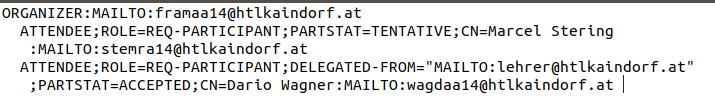
\includegraphics[width=\textwidth]{images/iCal_Format_attendee}
    \caption{iCal ATTENDEE Beispiel}
    \label{fig:netFramework}
\end{figure}
\subsection{TRANSP}
\label{sec:transp}
Diese Eigenschaft ist zur Angabe, ob ein Event beim Filtern nach ''beschäftigter Zeit'' angezeigt werden soll oder nicht. Der Wert der Eigenschaft TRANSP kann entweder ''OPAQUE'' oder ''TRANSPARENT''. Opaque bedeutet undurchsichtig und wird somit beim Filtern nach beschäftigter Zeit angezeigt.
%VALARM
\subsection{TRIGGER}
\label{sec:trigger}
\textbf{Anwendbar in:} VALARM \\
Gibt an wann ein Alarm ausgelöst werden soll. Der Standard-Wert ist die Eigenschaft ''DURATION'' \ref{sec:duration}. Es gibt mehrere Möglichkeiten anzugeben wann der Alarm ausgelöst werden soll. 
\begin{enumerate}
\item Trigger welcher 20 Minuten nach Start des Events auslöst: \\TRIGGER:-P20M\\
\item Trigger welcher 10 Minuten nach Ende des Events auslöst: \\TRIGGER;RELATED=END:P10M\\
\item Trigger welcher an einer absoluten Uhrzeit auslöst (17.03.2019 - 12 Uhr): \\TRIGGER;VALUE=DATE-TIME:20190317T120000Z\\
\end{enumerate}
\subsection{REPEAT}
\label{sec:repeat}
\textbf{Anwendbar in:} VALARM \\
Gibt an wie oft ein Alarm nach erstmaliger Auslösung wiederholt werden soll. Um einen Alarm mit 5 Minuten Abstand 4 mal zu wiederholen muss die REPEAT Eigenschaft wie folgt aussehen: \\ \\ REPEAT:4\\DURATION:PT5M
\renewcommand{\theauthor}{Dario Wagner}
\subsection{DURATION}
\label{sec:duration}
\textbf{Anwendbar in:} VEVENT, VTODO, VALARM, VFREEBUSY\\
Diese Eigenschaft gibt eine Dauer an. Bei einem Event kann sie eine Zeit angeben wie lange das Event dauert, anstatt einer DTEND Eigenschaft \ref{sec:dtend}. Die DURATION kann auch wie bei dem Beispiel einer REPEAT Eigenschaft \ref{sec:repeat} genutzt werden.
\subsection{ACTION}
\label{sec:action}
\textbf{Anwendbar in:} VALARM \\
Beschreibt die Aktion die ausgeführt wird wenn ein Alarm ausgelöst wird. Wie bei VALARM \ref{sec:vAlarm} beschrieben kann hier zum Beispiel ''ACTION:AUDIO'' angegeben werden, dann wird beim auslösen des Alarm ein Ton abgespielt. Welches Geräusch abgespielt wird hängt vom Verweis auf die Sound-Datei ab. 
\subsection{ATTACH}
\label{sec:attach}
\textbf{Anwendbar in:} VEVENT, VTODO, VALARM, VJOURNAL\\
Mithilfe der ATTACH-Eigenschaft kann eine Datei dem Termin angehängt werden. Dies könnte zum Beispiel ein wichtiges Formular für ein Meeting oder Notizen für eine Präsentation sein. 
\pagebreak